%!TEX root = ../dokumentation.tex

\begin{titlepage}
	\begin{longtable}{p{11.2cm} p{5.4cm}}
		{\raisebox{\ht\strutbox-\totalheight}{
\includegraphics[height=2.5cm]{images/dhbw.png}}} &
		% {\raisebox{\ht\strutbox-\totalheight}{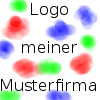
\includegraphics{images/firma-deckblatt.png}}}
	\end{longtable}
	\enlargethispage{20mm}
	\begin{center}
    \doublespacing{
		\vspace*{12mm}	{\LARGE\textbf \titel }}\\
		\vspace*{12mm}	{\large\textbf \arbeit}\\
		\vspace*{12mm}
		\vspace*{12mm}	\langartikelstudiengang{} \langstudiengang{} \studiengang\\
    \vspace*{0mm}		\langanderdh{} \dhbw\\
		\vspace*{12mm}	\langvon\\
		\vspace*{3mm}		{\large\textbf \autor}\\
		\vspace*{12mm}	\datumAbgabe\\
	\end{center}
	\vfill
	\begin{spacing}{1.2}
	\begin{tabbing}
		mmmmmmmmmmmmmmmmmmmmmmmmmm             \= \kill
		\textbf{\langdbbearbeitungszeit}       \>  \zeitraum\\
		\textbf{\langdbkurs}  \>  \kurs\\
		\textbf{\langdbbetreuer}               \>  \betreuer\\
	\end{tabbing}
	\end{spacing}
\end{titlepage}
